A lo largo del estado de la cuestión, será necesario abordar los campos relevantes de la psicología, la música y los videojuegos para fundamentar el desarrollo de la aplicación con investigaciones pertinentes. A continuación, se detallan los campos de interés que contribuirán a alcanzar los objetivos de la investigación.

\section{Marco teórico del trabajo}

\subsection{Ritmo, creación musical y emociones}

\subsubsection{Definición de ritmo y efectos terapéuticos}

El ritmo es un elemento intrínseco de la vida humana. Se manifiesta en la mayoría de las formas de arte, siendo de gran importancia en la música, la poesía y la danza. La definición de ritmo según \citeauthor{CONCEPTO:2021} (\citeyear{CONCEPTO:2021}) es la siguiente:

\begin{adjustwidth}{100pt}{0pt}
	''\textit{Se denomina ritmo a todo movimiento regular y recurrente, marcado por una serie de eventos opuestos o diferentes que se suceden en el tiempo. Dicho en otras palabras, el ritmo es un fluir del movimiento de naturaleza visual o sonora, cuyo orden interno puede percibirse e incluso reproducirse.}''
\end{adjustwidth}

La percepción del ritmo es totalmente subjetiva, pero para comprenderlo es esencial encontrar la clave que lo hace común para todos los individuos de la sociedad. Un ritmo siempre será un ritmo si los eventos que ocurren en el tiempo definen un patrón y un margen de repetición. Existen distintos tipos de ritmo en varias áreas artísticas. Sin embargo, nos centraremos en el ritmo musical, que es el más relevante para el campo psicológico de la musicoterapia. El ritmo musical se compone de varios elementos que indican su velocidad, intensidad y duración. El pulso, el tempo y la métrica son los elementos principales que definen un ritmo musical. Abordaremos individualmente cada uno de estos términos, indagando en profundidad que función tienen dentro de la música.

\begin{itemize}
	\item \textbf{Pulso:} es considerado como el latido del corazón de la música. Por definición, el pulso consiste en una serie de pulsaciones que se repiten de manera constante en una pieza musical, vinculadas directamente al movimiento del pie al escuchar una canción. El pulso puede tener diferentes velocidades, ya sean más rápidas o más lentas, pero siempre es constante a lo largo de la pieza musical. Sin embargo, existen excepciones si el compositor de la música decide acelerar o disminuir la velocidad intencionalmente (\cite{VIOLÍNZN:2024}).
	\item \textbf{Tempo:} proveniente del italiano ''tiempo'', el tempo se refiere a la velocidad de una composición. Metafóricamente, es similar a un reloj, que nos indica cuándo realizar ciertas acciones. El tempo permite a los músicos conocer el momento preciso en el que tocar cada sección de una pieza musical. Cuando los pulsos están distanciados equitativamente en el tiempo, la unidad de medida del tempo son BPM (\cite{MASTEREDBLOGS:2021}). El tempo puede ser constante, como en algunas canciones contemporáneas, o variable. Es común encontrar movimientos con distintos tempos en las piezas clásicas.
	\item \textbf{Métrica:} en el punto medio entre los dos términos anteriores, encontramos la métrica. Esta combina ambos elementos y define la estructura de una composición musical. La métrica se refiere a cómo se organizan los pulsos y el tempo en una pieza musical, agrupando los pulsos en unidades llamadas compases. En cada compás, algunos pulsos sonarán más fuertes y otros más suaves, lo cual se conoce como acentuación. La combinación de todos estos elementos proporciona un sentido rítmico a la música (\cite{COMPOMUSICAL:2024}). La métrica incorpora todas las figuras necesarias (\autoref{fig:MusicalFigures}) para visualizar la música en una partitura. La música se percibirá de manera diferente dependiendo de la altura, duración y tipo de figura que contengan la combinación de compases que conforman la pieza.
\end{itemize}

\begin{figure}[h!]
	\centering
	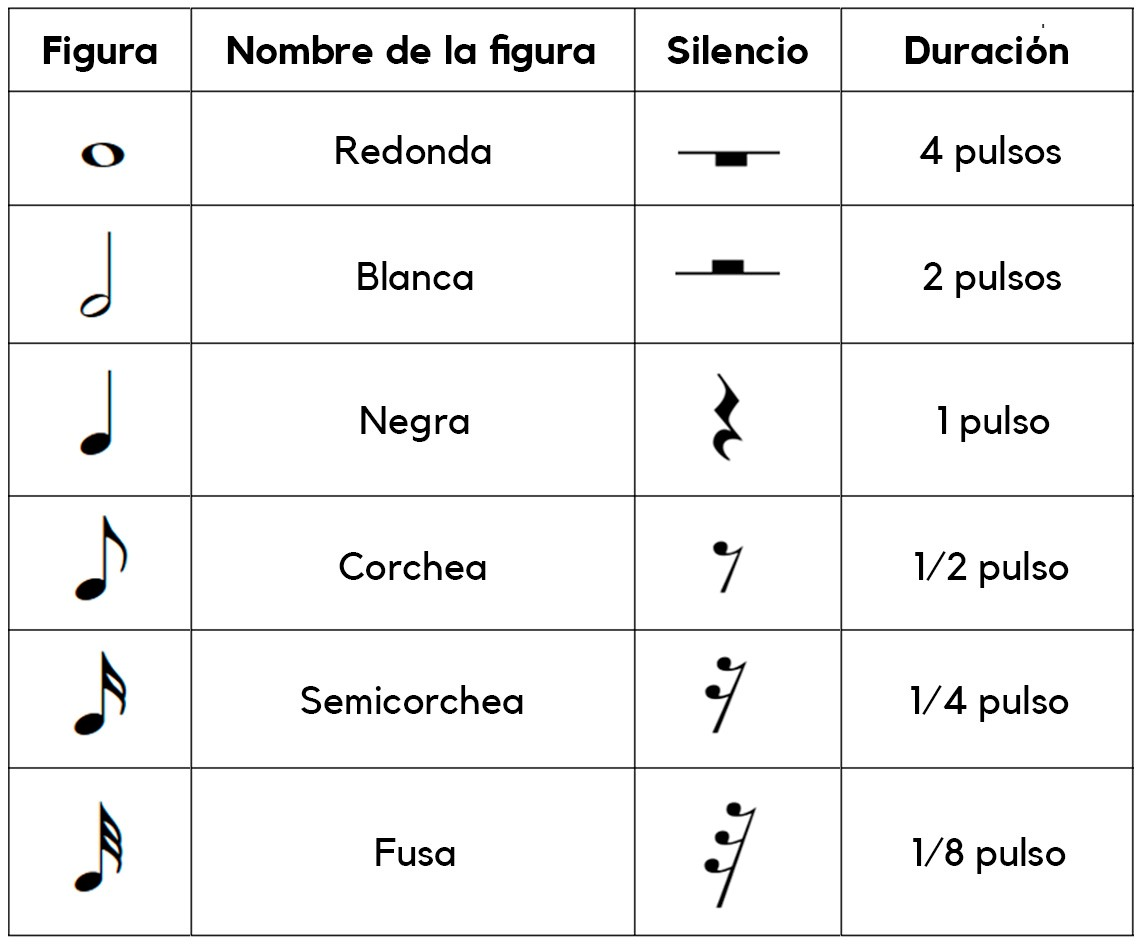
\includegraphics[width=0.4\linewidth]{Figuras/Estado/FigurasMusicales.jpg}
	\caption{Figuras musicales, incluyendo detalles sobre su nombre, duración, y la figura de silencio correspondiente.}
	\label{fig:MusicalFigures}
	\vspace{-35pt}
\end{figure}

\begin{center}
	\textbf{Fuente:} \citeauthor{VIOLÍNZN:2024} (\citeyear{VIOLÍNZN:2024}).
\end{center}

El ritmo tiene potencial terapéutico, ya que puede generar efectos positivos en el cuerpo y la mente. Según \citeauthor{JARAH:1977} (\citeyear{JARAH:1977}), el núcleo de un ritmo se define por dos fases: movimiento y ausencia de movimiento. A nivel fisiológico, estas dos fases están directamente relacionadas con la tensión y relajación. Aunque medir la música en función del tiempo puede ser deshumanizante, debemos hacerlo para facilitar la adaptación del intérprete a la pieza. La medición del tiempo en la música se hace de manera cíclica. Por eso, el ritmo es un elemento cíclico, ya que la mayoría de nuestras acciones dependientes del tiempo tienen esta propiedad. La respiración, una acción cíclica definida por la inhalación y la exhalación (Arsis y Tesis en términos musicales\footnote{Arsis y Tesis son las partes más fuerte y más débil de un compás musical, respectivamente. Se utilizan tanto en música como en poesía. Se definen en función de la dirección de la línea melódica y la duración de la última nota del compás con respecto al tono semifuerte (\cite{CASTELLANOS:2009})} (\cite{CASTELLANOS:2009})), es la acción humana cíclica más relevante. 

Entre los efectos terapéuticos que incluye el ritmo podemos encontrar la mejora de la coordinación motora, que ayuda a incrementar la sincronización de los pacientes, y la regulación emocional, promoviendo la calma con ritmos lentos o estimulando la energía con ritmos rápidos. Un ejemplo clínico del uso del ritmo se puede observar en un estudio realizado por \citeauthor{BENSIMON:2008} (\citeyear{BENSIMON:2008}), que muestra cómo los soldados de guerra con trastorno de estrés postraumático (TEPT), que presentan síntomas de soledad y aislamiento social, entre otros, se benefician de terapias de grupo. El ritmo es el elemento principal para su mejoría.

\subsubsection{Proceso de composición, formas y tipos}

Según \citeauthor{RAE:2024} (\citeyear{RAE:2024}), el término ''creación'' se refiere a la acción y efecto de crear. El acto de crear es muy amplio, ya que se puede adaptar a cualquier circunstancia en la que se genere algo de la nada. En nuestro contexto de estudio, la creación o composición musical consiste en organizar sonidos y silencios para transmitir emociones y expresar ideas (\cite{MMARTIN:2024}). Por lo tanto, la creación e invención musical es el punto culminante de la actividad creativa musical (\cite{SUBIRATS:2004}). La selección del ritmo, la melodía, la armonía y la textura son algunos de los elementos fundamentales para la composición musical. Para entender el proceso de composición, debemos considerar los niveles de creatividad de la mente humana. Según \citeauthor{SUBIRATS:2004} (\citeyear{SUBIRATS:2004}), existen cinco niveles, que se describen de la siguiente manera:

\begin{itemize}
	\item \textbf{Creatividad expresiva:} es la forma más básica de creación. Se basa en el descubrimiento de nuevas formas de expresar sentimientos, permitiendo al individuo identificarse con su propia obra y mejorar su comunicación con los demás. Además, es la forma de creación más presente en cualquier campo de expresividad como la música, la poesía o la danza. 
	\item \textbf{Creatividad productiva:} este tipo de creatividad se centra en la aplicación de técnicas y estrategias que ayudan al individuo a alcanzar un objetivo previamente fijado. Está orientada hacia la eficiencia de productividad, especialmente en situaciones que requieren la producción a gran escala.
	\item \textbf{Creatividad incentiva:} entre la expresividad (espontaneidad) y la producción (presupuestos), surge la creatividad incentiva, que se caracteriza por una mayor capacidad para descubrir nuevas realidades. En este caso, el ambiente juega un papel determinante.
	\item \textbf{Creatividad innovadora:} permite al individuo lograr resultados únicos a través de la transformación del medio. Supone una mayor flexibilidad de invención y mejora las capacidades creadoras del individuo.
	\item \textbf{Creatividad emergente:} esta cualidad define al genio que posee un gran talento a nivel creativo. No se trata de producir basándose en modificaciones de productos antiguos, sino que la creación de ideas se fundamenta en principios completamente nuevos.
\end{itemize}

La composición musical reúne todos estos niveles de creatividad. Existen dos formas de crear en este ámbito: la improvisación libre y la composición guiada. Cuando nos referimos a la improvisación libre, no hablamos de cualquier tipo de improvisación. Comúnmente, se entiende la improvisación como el acto de "tocar cualquier cosa". \citeauthor{OLMEDO:2014} (\citeyear{OLMEDO:2014}) define este tipo de improvisación con la frase: "Hay pacientes que improvisan pero no le doy estatuto de improvisación porque tocan de un modo maquinal y no escuchan". Sin embargo, la improvisación libre requiere un nivel de profundidad adicional del individuo. Debe entender las bases fundamentales de lo que está haciendo y por qué lo está haciendo, sin desviarse de las funciones de la improvisación. Además, la creación musical puede desarrollarse a través de varios formatos, dependiendo del instrumento que genera la música. La voz, objetos cotidianos o instrumentos musicales son los principales medios para la creación o composición musical.

\subsubsection{Relación entre la música y las emociones}

Las emociones y la música están estrechamente relacionadas. Aunque los gustos musicales son totalmente subjetivos, ciertos tipos de música provocan, en niveles distintos, las mismas emociones en todos los seres humanos. Normalmente, el cerebro funciona por regiones, activando ciertas áreas según la acción que se esté realizando. Sin embargo, la escucha activa de la música no parece activar ninguna zona específica, sino que se distribuye por todo el cerebro. Por lo tanto, cuando las personas reaccionan al estímulo de la música, experimentan diferentes sensaciones en el cuerpo. Esto se debe a que la música provoca un cambio tanto fisiológico como psicológico, una reacción conocida como biomúsica (\cite{MOSQUERA:2013}).

Un estudio realizado por \citeauthor{MOSQUERA:2013} (\citeyear{MOSQUERA:2013}), observó que al escuchar música agradable, se pueden activar ciertas sustancias químicas en el Sistema Nervioso Central. Esto estimula la producción de neurotransmisores como la dopamina, las endorfinas y la oxitocina, y se experimenta un estado que favorece la alegría y el optimismo en general. Sin embargo, la respuesta emocional puede variar entre individuos, ya que se refleja en función de las experiencias personales y aprendizajes previos de cada uno.

La expectativa musical desempeña un papel crucial en la gestión de emociones, ya que puede generar satisfacción o frustración, dependiendo de cada individuo y sus previsiones. En la expectativa musical, los oyentes formulan una serie de hipótesis sobre cómo continuará una pieza musical desde que suena la primera nota. Estas expectativas se fundamentan en una serie de teorías que \citeauthor{SENABRE:2019} (\citeyear{SENABRE:2019}) describe de la siguiente manera:

\begin{itemize}
	\item \textbf{Teoría sobre las Expectativas de Leonard B. Meyer:} la respuesta emocional del oyente puede interpretarse como resultado de las desviaciones en los eventos percibidos respecto a las normas estilísticas. El incumplimiento de la norma puede ser un estímulo que provoca la respuesta emocional del oyente.
	
	\begin{adjustwidth}{100pt}{0pt}
		\textit{''El disfrute provocado por la escucha musical surge de la percepción del juego del artista con formas y convenciones que están arraigadas como hábitos de percepción tanto en el artista como en el público. (…) No consiste en un interés intelectual en detectar semejanzas y diferencias, sino en el inmediato goce estético que resulta de la aparición y la suspensión o el cumplimiento de expectativas que son producto de muchos encuentros previos con obras de arte.''}
		\begin{flushright}
			\vspace{-10px}
			(\cite{MEYER:1956})
		\end{flushright}
	\end{adjustwidth}
	
	\item \textbf{Modelo de Implicación-Realización de Narmour:} el trabajo que Meyer comenzó fue continuado por Eugene Narmour, lo que permitió la comprobación empírica de algunos de sus aspectos. Este modelo sugiere que durante la escucha, se generan dos fuentes de expectativas asociadas a los dos sistemas de implicación melódica. De manera directa se hace alusión a los dos tipos de procesos que intervienen en la percepción: uno ascendente (procesos guiados por datos) y uno descendente (procesos guiados conceptualmente).
	\item \textbf{Modelo de Alfabetos de Deustch y Feroe:} Diana Deustch y John Feroe propusieron una teoría para formalizar cómo los oyentes representamos temporalmente las secuencias de alturas en la música tonal occidental, y cómo utilizamos esas representaciones para prever su continuación. Utilizaron un sistema de alfabeto para definir los distintos niveles de comprensión de la música. En la base de su alfabeto se encuentra la escala cromática.
	\item \textbf{Fuerzas Musicales de Steve Larson:} \citeauthor{LARSON:2002} (\citeyear{LARSON:2002}) propone una teoría en la que tres fuerzas, similares a las que inciden en los movimientos en el espacio físico, condicionan el comportamiento de los patrones musicales. Según la teoría de las fuerzas musicales, los oyentes anticipamos que la gravedad, el magnetismo y la inercia influirán en la continuidad de las secuencias escuchadas, generando la expectativa de una resolución completa.
	\item \textbf{Teoría de la Atención Dinámica de Mari R. Jones:} a diferencia de las teorías anteriores, la teoría de la Atención Dinámica propone un enfoque que pueda modelar la percepción y nuestras expectativas poniendo especial énfasis en el carácter dinámico de esta capacidad humana.
	
	\begin{adjustwidth}{100pt}{0pt}
		\textit{''La estructura del mundo es producto de nuestra capacidad para detectar cambios a lo largo de las dimensiones físicas (es decir, valores contrastantes) y de nuestra tendencia a representar estos cambios como relaciones a lo largo de dimensiones subjetivas.''}
		\begin{flushright}
			\vspace{-10px}
			(\cite{JONES:1976})
		\end{flushright}
	\end{adjustwidth}
\end{itemize}

La combinación de las experiencias personales y el aprendizaje previo de cada individuo conforman sus distintas reacciones al escuchar música y sus respectivas evocaciones emocionales. Es muy importante comprender a nivel de educación musical estos aspectos para poder gestionar las emociones de manera efectiva.

\subsection{Musicoterapia y ansiedad}

\subsubsection{Definición de ansiedad}

La ansiedad es una emoción que todos experimentamos en menor o mayor medida en algunos momentos de nuestra vida. Es una respuesta natural del cuerpo ante situaciones de peligro o estrés y puede manifestarse de varias formas. La ansiedad se define generalmente como un sentimiento de miedo, preocupación o malestar relacionado con eventos futuros inciertos. Fisiológicamente, la ansiedad activa el sistema nervioso simpático, desencadenando respuestas corporales como aumento del ritmo cardíaco, sudoración y tensión muscular (\cite{APA:2013}). Emocionalmente, puede provocar sensaciones de temor, y cognitivamente, puede conducir a pensamientos intrusivos acerca de posibles peligros o fracasos.

Según la American Psychological Association (\citeyear{APA:2020}), la ansiedad es distinta al miedo, ya que esta última es una respuesta a una amenaza inmediata, mientras que la ansiedad implica la anticipación a una amenaza futura. La ansiedad es un estado emocional que prepara a la persona para enfrentar potenciales peligros. Esta respuesta puede ser adaptativa cuando se presenta en niveles moderados, ya que puede mejorar el rendimiento y la atención. Sin embargo, si la ansiedad es excesiva y persistente, puede interferir de manera significativa en la vida diaria de una persona. En este último caso, sería crucial consultar a un especialista para identificar el grado de ansiedad que sufre la persona y tratarla de manera adecuada.

Los síntomas de la ansiedad se pueden clasificar en tres dimensiones: físicas, emocionales y cognitivas. Los síntomas físicos incluyen palpitaciones, sudoración, temblores, tensión muscular, dificultad para respirar, mareos, fatiga y problemas gastrointestinales. Son el resultado de la activación del sistema nervioso simpático, que prepara al cuerpo para la lucha o huida en situaciones percibidas como peligrosas (\cite{CRASKE:2016}). A nivel emocional, las personas con ansiedad a menudo experimentan una sensación constante de miedo o preocupación. Es posible que se sientan inquietos, irritables y que perciban una pérdida de control sobre sus emociones (\cite{BARLOW:2002}). En relación a los síntomas cognitivos, la ansiedad puede alterar la forma en que las personas piensan, provocando pensamientos intrusivos, preocupaciones excesivas y dificultades para concentrarse. Estos síntomas cognitivos pueden perpetuar el ciclo de ansiedad. La preocupación constante sobre posibles peligros puede intensificar los síntomas físicos y emocionales (\cite{CLARK:2011}). Todos estos síntomas pueden presentarse simultáneamente, complicando la vida cotidiana de quienes padecen ansiedad. Los niveles de ansiedad están directamente relacionados con la tolerancia de la persona y las circunstancias que rodean la aparición de estos síntomas.

\subsubsection{Tipos de trastornos de ansiedad}
Existen varios tipos de trastornos de ansiedad, cada uno con sus características y criterios diagnósticos propios. Los trastornos de ansiedad más comunes incluyen:

\begin{itemize}
	\item \textbf{Trastorno de Ansiedad Generalizada (TAG):} se caracteriza por una preocupación excesiva e incontrolable en relación con diversas actividades o eventos. Esto se acompaña de síntomas físicos como tensión muscular y problemas de sueño. Las personas con este trastorno suelen anticipar desastres y están constantemente preocupadas por su salud, dinero, familia o trabajo (\cite{APA:2013}).
	\item \textbf{Trastorno de pánico:} este trastorno se caracteriza por ataques de pánico recurrentes e inesperados. Estos son episodios de intenso miedo acompañados de síntomas físicos severos, que incluyen palpitaciones, sudoración, temblores y sensación de asfixia. Las personas con trastorno de pánico a menudo viven con el temor constante de sufrir más ataques. Esto puede llevarlas a evitar situaciones o lugares donde han experimentado ataques anteriormente (\cite{KESSLER:2005}).
	\item \textbf{Trastorno de ansiedad social:} también conocido como fobia social, este trastorno implica un temor intenso y persistente a ser juzgado, avergonzado o humillado en situaciones sociales o de desempeño. Las personas con trastorno de ansiedad social pueden evitar las interacciones sociales o soportarlas con gran angustia (\cite{STEIN:2008}).
	\item \textbf{Trastorno Obsesivo-Compulsivo (TOC):} aunque el TOC se clasifica de manera independiente en el DSM-5\footnote{El DSM-5, actualizado en 2013, es el Manual Diagnóstico y Estadístico de los Trastornos Mentales. Su objetivo es asistir a los profesionales de la salud en el diagnóstico de los trastornos mentales de los pacientes.}, está estrechamente relacionado con los trastornos de ansiedad. Este trastorno se caracteriza por pensamientos obsesivos intrusivos y comportamientos compulsivos repetitivos, los cuales están destinados a reducir la ansiedad causada por estas obsesiones (\cite{APA:2013}).
	\item \textbf{Trastorno de Estrés Postraumático (TEPT):} este trastorno se desarrolla después de que una persona ha sido expuesta a un evento traumático. Los síntomas incluyen la experimentación del trauma a través de flashbacks y pesadillas, la evitación de los recordatorios del evento, y un aumento de la excitabilidad o reactividad (\cite{YEHUDA:2002}).
	\item \textbf{Trastorno de ansiedad por separación:} es más frecuente en niños, pero también puede afectar a adultos. Se caracteriza por un miedo excesivo a la separación de las personas a las que el individuo está apegado. Los síntomas pueden incluir una angustia extrema al anticipar o experimentar la separación, así como preocupaciones constantes de que algo malo suceda a la persona a la que está apegado (\cite{APA:2013}).
	\item \textbf{Fobias específicas:} las fobias son miedos intensos e irracionales hacia objetos o situaciones específicas, como por ejemplo, las alturas, los animales o volar. Estos miedos exagerados pueden provocar una evitación extrema de los estímulos que los causan e interferir significativamente en la vida diaria de una persona (\cite{APA:2013}).
\end{itemize}

A pesar de que los trastornos de ansiedad representan el mayor problema de salud mental en los EE. UU, la mayoría de las personas nunca buscan ayuda médica. Estos muestran una etiología compleja, donde se reconoce el componente genético y los factores estresantes debido a los acontecimientos de la vida. Para su diagnóstico, los médicos y psiquiatras se basan en los criterios clínicos establecidos por el Manual Diagnóstico
y Estadístico de los Trastornos Mentales (DSM-5) (\cite{DELGADO:2021}).

\subsubsection{Terapias tradicionales para la ansiedad}

Para tratar la ansiedad se emplean diversas terapias tradicionales, las cuales han demostrado ser efectivas para las afecciones físicas y psicológicas de los pacientes. Estas se pueden clasificar en terapias psicológicas y tratamientos farmacológicos. Para decidir qué tratamiento utilizar, es necesario realizar una evaluación previa para identificar el tipo de trastorno que tiene el paciente. Aunque ambas opciones se utilizan para tratar la ansiedad, las terapias se consideran tratamientos de primera línea. Estas se combinan para modular los patrones de pensamiento (\cite{DELGADO:2021}).

Las terapias psicológicas son intervenciones respaldadas por evidencia que se enfocan en cambiar los patrones de pensamiento y comportamiento que contribuyen a la ansiedad. Entre las más efectivas están la terapia cognitivo-conductual (TCC), la terapia de exposición, y la terapia de aceptación y compromiso (ACT). Estas terapias no sólo funcionan y se utilizan individualmente, sino que también ofrecen la posibilidad de ser utilizadas de manera complementaria. De esta forma, el terapeuta puede aprovechar las virtudes de cada una para obtener los resultados requeridos en los objetivos terapéuticos.

La TCC es ampliamente reconocida como una de las terapias más efectivas para tratar la ansiedad. Esta se centra en identificar y transformar patrones de pensamiento negativos y comportamientos disfuncionales que alimentan la ansiedad. Los pacientes aprenden técnicas de afrontamiento y estrategias de relajación para manejar su ansiedad de manera más efectiva (\cite{HOFMANN:2012}).

La terapia de exposición, como sugiere su nombre, implica exponer al paciente gradualmente a los estímulos que le causan 	ansiedad en un entorno controlado. El objetivo es disminuir la sensibilidad del paciente, reduciendo su respuesta de ansiedad. La exposición puede ser en vivo, donde el paciente enfrenta directamente la situación temida, o imaginaria, donde visualiza la situación (\cite{CRASKE:2008}). Esta terapia es particularmente eficaz en el tratamiento de fobias específicas, trastorno de pánico y TEPT (\cite{POWERS:2010}).

En cuanto a la terapia ACT, esta se enfoca en aceptar pensamientos y sentimientos difíciles en lugar de resistirse a ellos. Además, promueve el compromiso con acciones que estén en línea con los valores personales del paciente. Esta terapia ayuda a los pacientes a llevar una vida significativa a pesar de la ansiedad, fomentando la flexibilidad psicológica (\cite{HAYES:2012}).

En relación con los tratamientos farmacológicos, estos ayudan a manejar los síntomas de la ansiedad. Los antidepresivos, particularmente los inhibidores selectivos de la recaptación de serotonina (ISRS) y los inhibidores de la recaptación de serotonina y norepinefrina (IRSN), son comúnmente usados para tratar la ansiedad. Estos medicamentos incrementan los niveles de neurotransmisores en el cerebro, lo cual mejora el estado de ánimo y reduce la ansiedad (\cite{BALDWIN:2014}). Por otro lado, los ansiolíticos como las benzodiazepinas proporcionan alivio rápido de los síntomas de ansiedad. No obstante, debido a su potencial de adicción y abuso, su uso generalmente se limita a corto plazo (\cite{FOND:2023}). Los betabloqueantes, como el propranolol, se utilizan para tratar los síntomas físicos de la ansiedad, como taquicardia y temblores. Estos medicamentos bloquean los efectos de la adrenalina, ayudando a reducir los síntomas físicos (\cite{STEENEN:2016}).

\subsubsection{Definición de musicoterapia}

La World Federation of Music Therapy (WFMT) define la musicoterapia de la siguiente manera; citamos literalmente: 

\begin{adjustwidth}{100pt}{0pt}
\textit{''La musicoterapia se refiere al uso profesional de la música y sus elementos como una intervención en entornos médicos, educativos y cotidianos con individuos, grupos, familias o comunidades que buscan optimizar su calidad de vida y mejorar su salud física, social, comunicativa, emocional, intelectual y espiritual. La musicoterapia se utiliza para satisfacer las necesidades físicas, emocionales, cognitivas y sociales de los pacientes}.'' \\
\begin{flushright}
	\vspace{-30px}
	(\cite{WFMT:2024})
\end{flushright}
\end{adjustwidth}

La música se ha utilizado como herramienta terapéutica durante muchos años. Como medio de expresión no verbal, la música facilita la comunicación y la exteriorización de sentimientos, permitiendo a las personas explorar o reexplorar su interior y compartirlo con los demás. El objetivo de usar música es facilitar la expresión emocional del individuo y su desarrollo comunicativo (\cite{TRESIERRA:2005}). Es importante incorporar la música en la educación emocional, especialmente en los niños. Debemos inculcar la importancia de la música como una herramienta en sus vidas que les ayude a gestionar sus emociones. Según \citeauthor{POCH:2001} (\citeyear{POCH:2001}), la música no debe considerarse superflua, ya que ofrece una serie de aportaciones más allá de ser simplemente un pasatiempo. La música tiene un impacto inmediato en los seres humanos, afectando aspectos biológicos, físicos, neurológicos, psicológicos, sociales y espirituales. Además, la música es un patrón autocurativo que la humanidad siempre ha utilizado. Por ejemplo, para aliviar tensiones, cubrir carencias afectivas o expresar sentimientos de alegría a través de la danza, el dolor de una muerte o el amor en canciones románticas. La música acompaña a una persona en todos los momentos esenciales de su vida. Esta presencia se ve reforzada por la cultura, que ha creado canciones y composiciones para cada uno de estos momentos.

La musicoterapia tiene aplicaciones en diversos campos psicológicos. Por ejemplo, en la Unidad de Cuidados Intensivos (UCI) Pediátrica, \citeauthor{TRESIERRA:2005} (\citeyear{TRESIERRA:2005}) explica que la música actúa como un agente relajante, permitiendo al paciente comunicar sus emociones en un entorno donde se sienta escuchado. Además, el efecto relajante de la música está directamente relacionado con la percepción del dolor y el estrés, lo que puede tener un impacto positivo en el sistema inmunológico del paciente. Esta serie de reacciones en cadena mejora el bienestar biológico del paciente. Según \citeauthor{TRESIERRA:2005} (\citeyear{TRESIERRA:2005}), las terapias para niños autistas pueden beneficiarse de la musicoterapia. Esta puede romper el aislamiento social y mejorar el desarrollo socioemocional. En estos casos, un instrumento musical puede actuar como intermediario entre el paciente y el terapeuta, fortaleciendo su comunicación.

\subsubsection{Modalidades de musicoterapia}

La musicoterapia abarca diversos métodos y aplicaciones, agrupándose en dos modalidades distintas. La musicoterapia activa es aquella donde el paciente dirige la acción, combinándola normalmente con la creación musical como base fundamental. En contraste, la musicoterapia receptiva es aquella donde el paciente se convierte en un sujeto pasivo, como por ejemplo, escuchando cierto tipo de música relajante, y que impacta en sus emociones de manera inherente.

La musicoterapia activa conlleva que el paciente participe activamente en el proceso terapéutico, ya sea cantando, tocando un instrumento o bailando. En este escenario, el paciente se convierte en el intérprete o creador de la música, mientras que el terapeuta sirve como un acompañante del proceso. Un elemento crucial en la musicoterapia activa es la improvisación musical, la cual se define como el arte de crear música de manera espontánea al tocar. No se trata de crear música desde cero, sino más bien de responder a experiencias musicales previamente aprendidas. En estas terapias, el terapeuta no solo acompaña al paciente, sino que también puede participar activamente junto a él. Es fundamental que el terapeuta comprenda las intenciones creativas del paciente, ya que si no hay una conexión musical entre ambos, la musicoterapia activa no será efectiva (\cite{SALAMANCA:2003}).

En la musicoterapia receptiva o pasiva, dependiendo del contexto, a diferencia de la anterior modalidad, el paciente escucha música grabada o interpretada en vivo por el terapeuta. Aunque el paciente sigue participando en la sesión, su función cambia, convirtiéndose en un agente pasivo. Este tipo de musicoterapia puede aliviar el estrés y la ansiedad, mejorar la concentración y la creatividad, entre otros beneficios. Existen dos acercamientos comunes de la musicoterapia receptiva: el canto armónico y los cuencos tibetanos. El canto armónico es una hermosa forma de expresión que consiste en cantar dos, tres o incluso cuatro sonidos simultáneamente, utilizando la mayor cantidad posible de resonadores dentro del cuerpo y el cráneo. Por otro lado, los cuencos tibetanos están compuestos por hasta siete metales diferentes\footnote{Según las tradiciones, cada metal está relacionado con un astro diferente de nuestro sistema solar (\cite{SALAMANCA:2003}).}, que producen distintas resonancias armónicas. Estos cuencos, que se utilizan comúnmente para la meditación, se llenan con distintos niveles de agua para conseguir diferentes tipos de sonidos y efectos cuando se golpean o se frotan (\cite{SALAMANCA:2003}).

Como explica \citeauthor{BRUSCIA:1998-2} (\citeyear{BRUSCIA:1998-2}), en relación con ambas modalidades, cada sesión de musicoterapia involucra al paciente en algún tipo de experiencia musical. Estos diferentes tipos de experiencias musicales pueden incorporarse a las terapias de manera única o complementaria, según lo decida el terapeuta en función de las necesidades del paciente. Los cuatro tipos básicos son:

\begin{itemize}
	\item \textbf{Improvisación:} el paciente crea música ya sea cantando o tocando un instrumento de forma espontánea.
	\item \textbf{Recreación:} el paciente canta o toca una pieza musical preexistente, ya sea de memoria o con partitura.
	\item \textbf{Composición:} con la ayuda del terapeuta, el objetivo es componer y anotar una pieza musical en una partitura.
	\item \textbf{Escuchar:} el cliente escucha música, ya sea pregrabada o en vivo.
\end{itemize}

La improvisación, la recreación y la composición forman parte de la musicoterapia activa. Cada uno de estos enfoques ofrece una serie de beneficios únicos. Es útil implementar en la terapia cada uno de ellos de manera específica después de analizar el tipo de patología al que va dirigido. Sin embargo, la escucha es parte de la musicoterapia receptiva.

La música actúa como aliada en la terapia, colaborando con el terapeuta para intervenir conjuntamente. El terapeuta puede utilizar la música para alcanzar sus objetivos, ya sea por sí misma o en combinación con intervenciones personales. La naturaleza de las intervenciones musicales en la terapia puede variar según la estética que se desee transmitir al paciente. Sonido, belleza y creatividad se unen en la musicoterapia para ofrecer una metodología poderosa en la gestión emocional de los pacientes (\cite{BRUSCIA:1998-2}). Además, la musicoterapia es una opción poderosa en las terapias de grupo. Como explican \citeauthor{PRIETO:2022} (\citeyear{PRIETO:2022}), la música une a las personas sin importar la nacionalidad, el color o la raza. Contribuye a nuestra construcción y abre un camino de trascendencia más allá de nuestro cuerpo e intelecto. Independientemente de nuestra condición física o psicológica, la evocación emocional de la música es común a todas las personas.

\subsubsection{Beneficios de la musicoterapia en el tratamiento de la ansiedad}

La musicoterapia ha surgido como un tratamiento eficaz para gestionar la ansiedad, fundamentada por una creciente base de evidencia científica. Varios estudios y ensayos clínicos han demostrado que la musicoterapia puede disminuir significativamente los niveles de ansiedad en poblaciones de distintos contextos, desde pacientes hospitalizados hasta individuos con trastornos de ansiedad generalizados. Un estudio realizado por \citeauthor{SEPULVEDA:2014} (\citeyear{SEPULVEDA:2014}) en una población de niños de entre 8 y 16 años con diferentes tipos de cáncer, encontró una disminución significativa en los niveles de ansiedad tanto antes (prequimioterapia) como después (posquimioterapia) de la quimioterapia. No obstante, cuando se combinó esta terapia convencional con la escucha de música, la reducción en los niveles de ansiedad fue sustancialmente mayor. Para ser precisos, los niveles de ansiedad pasaron a reducirse del 27\% al 95\%.

\subsection{Videojuegos serios para la salud}

\subsubsection{Definción e historia de los videojuegos serios}

Los ''serious games'', o videojuegos serios, están diseñados con un propósito que va más allá del mero entretenimiento. Se utilizan en varios campos, como la educación, la salud, la formación militar y la simulación profesional, con el objetivo de alcanzar metas específicas en cada campo concreto. Estas pueden ser el desarrollo de habilidades, la alteración de comportamientos, o la terapia psicológica. A diferencia de los videojuegos tradicionales, que buscan principalmente entretener, los videojuegos serios tienen como objetivo educar, capacitar o generar cambios positivos en los usuarios.

Los videojuegos serios poseen una serie de características que los diferencian del formato convencional de los videojuegos, cuyo principal objetivo es entretener.

\begin{itemize}
	\item \textbf{Propósito educativo o terapéutico:} es evidente que el objetivo de los juegos serios es distintivo. A diferencia de los videojuegos convencionales, cuyo propósito es proporcionar entretenimiento, los juegos serios buscan impartir conocimientos o habilidades específicas a través de su diseño. Un estudio realizado por \citeauthor{GRAAFLAND:2012} (\citeyear{GRAAFLAND:2012}), analiza cómo los videojuegos serios pueden proporcionar un entorno seguro para que los profesionales practiquen cirugía en un entorno controlado sin poner en peligro a ningún paciente.
	\item \textbf{Interactividad:} al adaptarse al formato digital del videojuego convencional, la interacción con el medio ofrece un feedback inmediato. Como explican \citeauthor{CONNOLLY:2012} (\citeyear{CONNOLLY:2012}), esto permite que los usuarios aprendan rápidamente y sobre todo practicando en entornos cercanos a la realidad.
	\item \textbf{Enfoque en el usuario:} al estar completamente adaptados a las necesidades específicas del usuario, los videojuegos serios permiten una personalización que maximiza su efectividad para cumplir con su objetivo.
	\item \textbf{Evaluación y métricas:} el entorno digital permite realizar un seguimiento a tiempo real de las actividades del usuario. Además, la implementación de métodos para evaluar el progreso del usuario ofrecen al administrador la posibilidad de dirigir o ajustar las actividades según las necesidades que se observen. Este factor es crucial en entornos educativos y terapéuticos.
\end{itemize}

La historia de los videojuegos serios se remonta a la década de los años 60, con el desarrollo de simulaciones militares que buscaban entrenar a los soldados en tácticas y estrategias sin el riesgo de un combate real (\cite{SAWYER:2002}). Desde entonces, la evolución de estos juegos ha estado creciendo, expandiéndose a diversos campos y aprovechando los avances tecnológicos para crear experiencias cada vez más inmersivas y efectivas en su propio contexto. 

En la educación, los videojuegos serios comenzaron a ganar popularidad en la década de 1980 con juegos como \textit{The Oregon Trail} (\cite{OREGONTRAIL:1971}), que combinaba elementos de juego con lecciones de historia y supervivencia. En el ámbito de la salud, los años 2000 vieron un aumento en el desarrollo de juegos diseñados para la rehabilitación física y mental, como \textit{Re-Mission} (\cite{REMISSION:2006}), cuyo objetivo es ayudar a los pacientes jóvenes con cáncer a comprender y manejar su enfermedad. Hoy en día, los videojuegos serios utilizan tecnologías emergentes como la realidad virtual y aumentada para crear entornos de aprendizaje y terapia. Estas innovaciones permiten a los usuarios experimentar situaciones complejas y aprender de ellas en un entorno controlado y seguro (\cite{FREITAS:2011}).

\subsubsection{Aplicaciones de los videojuegos serios en el campo de la salud mental}

Los videojuegos serios poseen un enorme potencial como herramientas terapéuticas para la salud mental, gracias a sus características destacadas previamente. Pueden ayudar a mejorar las habilidades sociales, especialmente en personas con Trastornos del Espectro Autista (TEA) y otros trastornos del desarrollo. El objetivo de diseñar videojuegos serios en este contexto es fomentar la empatía, la comunicación y la colaboración a través de interacciones sociales simuladas. Los videojuegos que simulan diversas perspectivas y experiencias emocionales son buenos consiguiendo esto. Por ejemplo, \textit{The Sims 4} (\cite{SIMS4:2014}), aunque no es un videojuego serio en el sentido tradicional, se ha adaptado en ciertos estudios para ayudar a los jugadores a comprender y manejar las emociones de los personajes, mejorando así la empatía y la comprensión emocional (\cite{FERGUSON:2013}).

Otra área de aplicación de los videojuegos serios es en el ámbito del entrenamiento cognitivo. Estos pueden diseñarse para mejorar funciones cognitivas como la memoria, la atención y la resolución de problemas, que suelen verse presentes en personas con trastornos mentales o neurodegenerativos. Por ejemplo, \textit{CogniFit} (\cite{COGNIFIT:1999}) ofrece una serie de pequeños juegos basados en neurociencia que se utilizan para entrenar algunas de estas habilidades cognitivas. Estudios han demostrado que el uso regular de este tipo de  videojuegos puede conducir a mejoras significativas en la memoria y la atención en adultos mayores y personas con deterioro cognitivo leve (\cite{LAMPIT:2014}).

En relación con nuestra área de estudio concreta, el tratamiento de la ansiedad se aprovecha de la interacción de este formato digital para implementar ejercicios de respiración y meditación guiados. Según \citeauthor{BOUCHARD:2017} (\citeyear{BOUCHARD:2017}), las terapias que incorporan el formato de realidad virtual (VR) con elementos de relajación, aumentan su efectividad, reduciendo significativamente los niveles de ansiedad de los pacientes.

\subsubsection{Elementos de diseño de videojuegos serios para el tratamiento de la ansiedad}

Las terapias tradicionales para la ansiedad son enormemente compatibles con el diseño de videojuegos serios. Este formato digital, que permite utilizar técnicas para la exposición gradual, la relajación y la gestión del estrés, proporciona un entorno controlado para el paciente en el que pueda enfrentarse a sus miedos. Esta metodología se alinea con los objetivos y métodos de la teoría de la exposición, que como comentamos anteriormente, es una técnica muy utilizada en el tratamiento contra la ansiedad.	

El diseño de videojuegos serios para tratar la ansiedad debe contener elementos que promuevan la relajación y la reducción del estrés. Videojuegos como \textit{Journey} (\cite{JOURNEY:2012}) o \textit{Flower} (\cite{FLOWER:2009}) utilizan mecánicas de juego simplificadas y paisajes visualmente atractivos para inducir un estado de relajación y reducir los niveles de estrés. Además, el uso de la música y sonidos relajantes es un componente clave en el diseño de este tipo de videojuegos con un enfoque más terapéutico. En cuanto a la narrativa, el uso de historias que se centren en el autodescubrimiento personal y en el empoderamiento del paciente también pueden ayudar a mejorar la gestión de las emociones.

El feedback en este tipo de videojuegos es de mucha importancia. Se debe desarrollar en dos capas: una capa satisfactoria para el paciente y una útil para el terapeuta. La capa de satisfacción para le paciente debe incluir indicadores visuales y auditivos que muestran cómo el jugador está progresando en los ejercicios de respiración o meditación. Esto no solo ayuda a los pacientes a corregir y mejorar sus técnicas en tiempo real, sino que también puede proporcionar un sentido de logro y competencia, lo que es esencial para mantener la motivación y el compromiso (\cite{CONNOLLY:2012}). En cuanto a la capa de utilidad para el terapeuta, es importante que todos los datos de interacción queden registrados para el estudio del profesional al cargo de la terapia. Esto ayudará al terapeuta a saber cuál es el progreso del paciente, de manera que pueda reajustar las terapias si fuera necesario.

Otro elemento de diseño importante es la personalización y adaptabilidad. Es crucial que los terapeutas puedan ajustar los niveles de dificultad, los tipos de actividades terapéuticas y los contenidos específicos del videojuego según las necesidades de cada paciente (\cite{BOUCHARD:2017}). A nivel de usuario, permitir la personalización de colores, temas visuales o música puede aumentar la participación del paciente. Un estudio dirigido por \citeauthor{FREITAS:2011} (\citeyear{FREITAS:2011}), demostró que personalizar elementos en estos juegos puede incrementar la motivación del usuario. Sin embargo, es importante no dar al paciente total libertad de elección, ya que podría perderse la dirección de la terapia, interfiriendo con los objetivos principales.

\section{Trabajos relacionados}

A pesar de la abundancia de trabajos sobre la aplicación de videojuegos serios para la salud, ha sido difícil encontrar estudios centrados en terapias psicológicas basadas en musicoterapia para trabajar las emociones. Es aún más raro encontrar estudios de este tipo específicos sobre ansiedad. En los trabajos relacionados, exploraremos algunos videojuegos serios con enfoque en el tratamiento de alguno de los tipos de ansiedad.

\subsection{Operation Quest (\cite{OPERATIONQUEST:2024})}

Operation Quest es uno de los lanzamientos más recientes con respecto al desarrollo de videojuegos serios para la salud. Santiago de Matos de Lima y Lucía Zerbetto, desarrolladores del juego, nos deleitaron este año 2024 con una experiencia diseñada para pacientes infantiles que se someterán a procedimientos médicos, en especial, procedimientos quirúrgicos. El objetivo de la aplicación está en, mediante la narrativa y mecánicas, potenciar las mentes jóvenes y promover una actitud positiva, que pueda combatir contra la ansiedad que genera un preparatorio quirúrgico. Estos objetivos se cumplen mediante un desarrollo basado en la terapia de exposición. Normalmente, los niños tienen miedo de aquello que no conocen. Por eso, es importante explicarles en que consiste el procedimiento que se les va a realizar y otorgarles seguridad en un entorno familiar en el que puedan aprender.

\begin{figure}[h!]
	\centering
	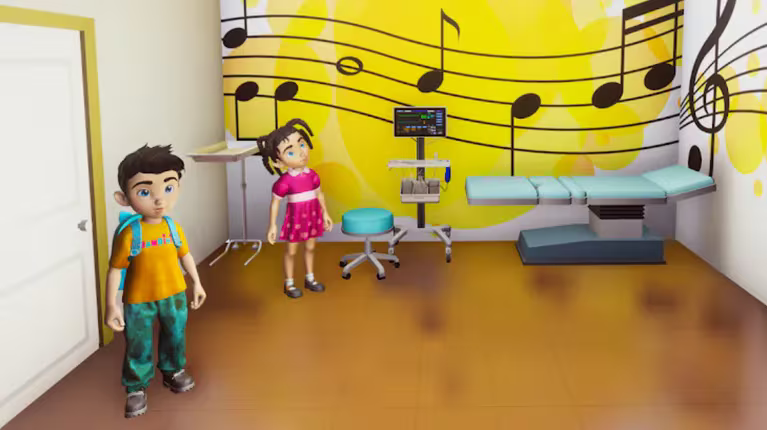
\includegraphics[width=0.55\linewidth]{Figuras/Estado/OperationQuest1.png}
	\caption{Captura de pantalla dentro del videojuego serio Operation Quest.}
	\label{fig:OperationQuest1}
	\vspace{-30pt}
\end{figure}

\begin{center}
	\textbf{Fuente:} Operation Quest (\citeyear{OPERATIONQUEST:2024}).
\end{center}

La idea del juego surgió durante la pandemia de COVID-19. Santiago de Matos de Lima, quien ha tenido un interés en el desarrollo de videojuegos desde la infancia, se percató de que la comunicación en línea entre profesionales era vital dada la situación del año 2020. Inicialmente, desarrollaron una aplicación para cumplir con este objetivo, pero acercándose las primeras bocanadas de aire tras la cuarentena evolucionó en lo que ahora conocemos como Operation Quest. Aprovechando la comunicación en línea, esta última versión permite que el médico pueda asistir al paciente mientras que tanto los pacientes como los familiares están jugando.

Operation Quest está directamente relacionado con proyecto ARTEMIS en varios aspectos. Su enfoque serio hacia la interacción digital orientada al público infantil lo convierte en una importante referencia para entender cómo se ha adaptado la interacción a este público. La función de doble usuario en la que el paciente y terapeuta están interactuando de manera simultánea, permite una comunicación fluida y mejora la eficacia de la terapia.

\subsection{SPARX (\cite{SPARX:2013})}

El videojuego serio SPARX (Smart, Positive, Active, Realistic \& X-factor thoughts) fue desarrollado por un grupo de investigadores de la Universidad de Auckland ubicada en Nueva Zelanda. Su objetivo es ayudar a jóvenes que sufren de ansiedad, estrés o depresión, utilizando como base la terapia cognitivo-conductual. Antes de su uso, es necesario realizar una evaluación para determinar si el caso específico del paciente es compatible con esta terapia digital.

Aunque su apartado gráfico no es especialmente cautivador, algo esperado debido a su fecha de publicación, la narrativa y el diseño sonoro son lo que definen este videojuego. La narrativa centrada en transmitir los mensajes a través de rompecabezas que fomentan la superación y motivación, hace que el jugador se sienta bien al resolverlos y comprenda su situación. Además, su diseño sonoro relajante hace que la experiencia de usar esta aplicación sea intrínsecamente calmante, proporcionando cierto alivio simplemente al usarla.

\begin{figure}[h!]
	\centering
	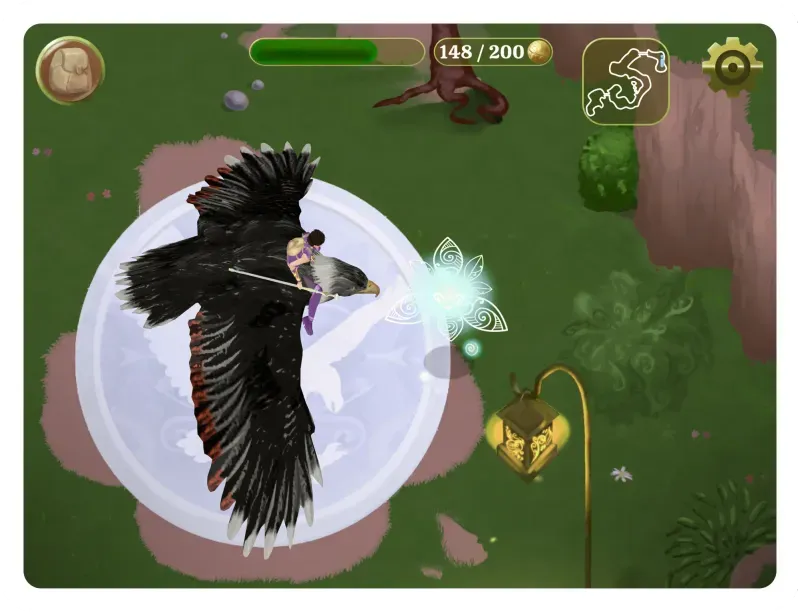
\includegraphics[width=0.5\linewidth]{Figuras/Estado/SPARX.png}
	\caption{Captura de pantalla dentro del videojuego serio SPARX.}
	\label{fig:SPARX}
	\vspace{-30pt}
\end{figure}

\begin{center}
	\textbf{Fuente:} SPARX (\citeyear{SPARX:2013}).
\end{center}

El proyecto ARTEMIS puede beneficiarse del videojuego SPARX en términos de narrativa. El juego anima al paciente a identificarse con el personaje principal y los NPCs respectivos, quienes le sitúan en contexto y le ayudan a entender lo que está ocurriendo. Además, el diseño sonoro natural, refinado para evocar emociones de tranquilidad y serenidad, es otro aspecto a considerar. La forma en que los rompecabezas se presentan al paciente y cómo se genera motivación para resolverlos también es un aspecto que podemos considerar para el desarrollo de la aplicación.

\subsection{Flow (\cite{FLOW:2006})}

Flow es uno de los pocos juegos que se han comercializado con un enfoque serio, representando perfectamente cómo se puede utilizar el medio interactivo digital para evocar sensaciones de relajación. Originalmente, Flow fue parte de la tesis doctoral de Jenova Chen, pero más tarde fue reinventado bajo la supervisión y financiación de SIE para PlayStation 3.

El diseño del juego se basa en la tesis de Jenova Chen, que se centra en el ajuste dinámico de la dificultad y en la teoría del psicólogo Mihaly Csikszentmihalyi sobre la inmersión mental, comúnmente conocida como teoría del flow. El videojuego creado por Chen, posee un apartado visual y auditivo que lo hace muy especial. El jugador controla una especie de serpiente que crece al alimentarse de partículas. Aunque las mecánicas del juego son simples, la relajante ambientación sumerge al jugador en un estado de calma, perpetuado por todos estos elementos.

\begin{figure}[h!]
	\centering
	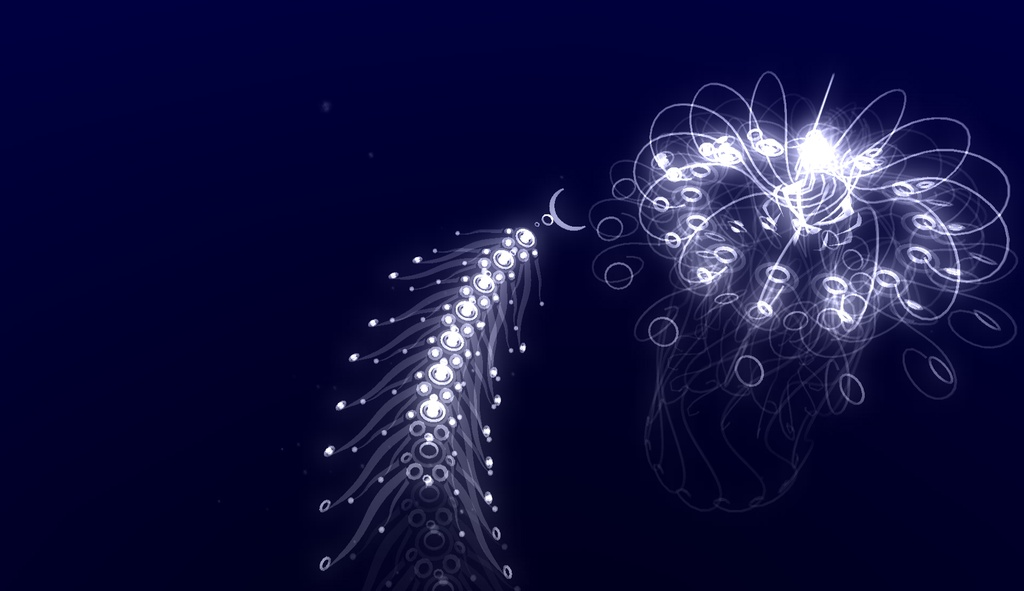
\includegraphics[width=0.6\linewidth]{Figuras/Estado/Flow.jpg}
	\caption{Captura de pantalla dentro del videojuego serio Flow.}
	\label{fig:Flow}
	\vspace{-30pt}
\end{figure}

\begin{center}
	\textbf{Fuente:} Flow (\citeyear{FLOW:2006}).
	
\end{center}

ARTEMIS se inspira en este videojuego por la simplicidad de sus mecánicas, lo que hace que la experiencia se centre en el disfrute intrínseco de los elementos que la componen, planteando un desafío subjetivo que el jugador se impone. Este reto aparece en forma de puzle de entorno, en el que la solución no está definida, sino que la define el propio jugador con su propia experiencia. La estética natural en la que las partículas florales forman una bella imagen, nos han permitido en nuestro desarrollo crear una sinergia entre lo visual y lo sonoro que evoque emociones de tranquilidad en el paciente, mediante su interacción con el entorno electrónico. 

\subsection{Deep VR (\cite{DEEP:2021})}

Deep VR es una experiencia de meditación en realidad virtual que se controla con la respiración del usuario. Utiliza un periférico que mide la dilatación del diafragma para precisar las dimensiones de las inhalaciones y exhalaciones. Los jugadores pueden navegar por un mundo subacuático controlando sus movimientos a través de la respiración profunda. El objetivo principal de la aplicación es reducir el estrés y aliviar la ansiedad.

\begin{figure}[h!]
	\centering
	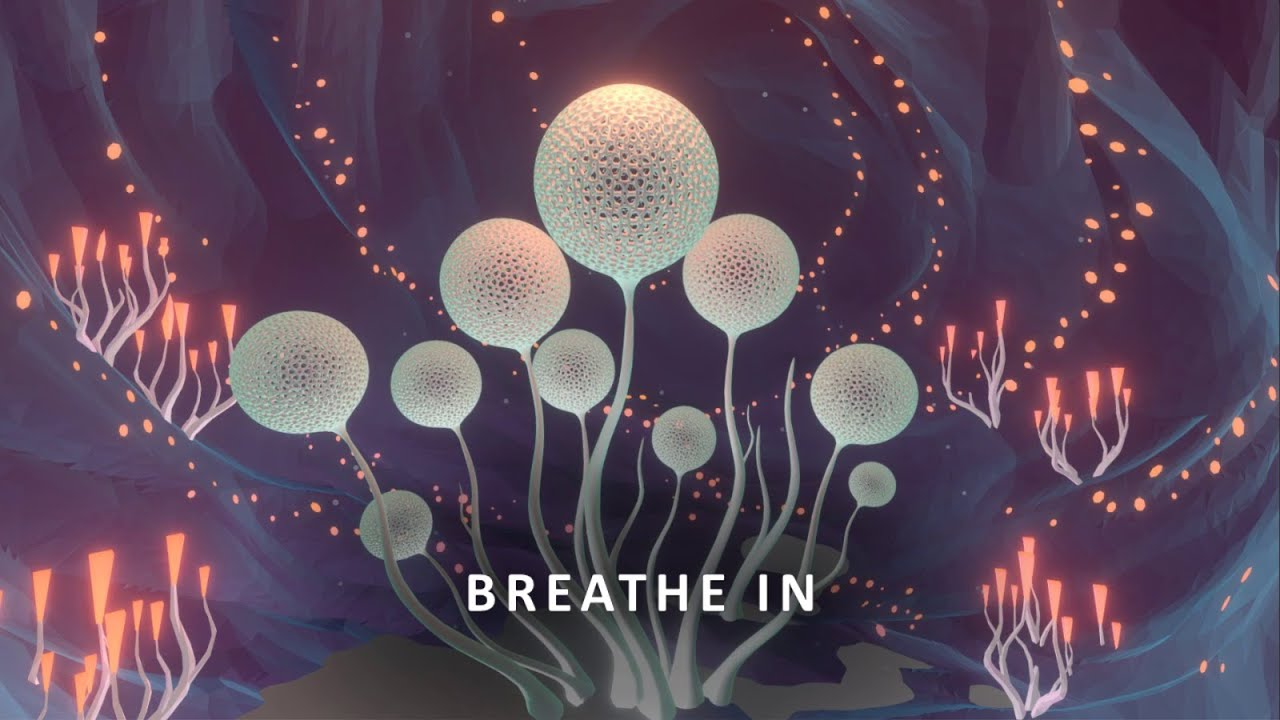
\includegraphics[width=0.8\linewidth]{Figuras/Estado/DeepVR.jpg}
	\caption{Captura de pantalla dentro del videojuego serio Deep VR.}
	\label{fig:DeepVR}
	\vspace{-30pt}
\end{figure}

\begin{center}
	\textbf{Fuente:} Deep VR (\citeyear{DEEP:2021}).

\end{center}

La combinación del formato de realidad virtual y el hermoso paisaje, junto con un diseño de audio mágico, facilita la inmersión en este mundo submarino. Todos estos elementos funcionan conjuntamente para conseguir el objetivo principal de esta experiencia; relajar al paciente.

Aunque el formato de Deep VR no es compatible con el proyecto ARTEMIS, su método de narración es útil. En particular, la forma en que la historia se cuenta a través del entorno, sin diálogo ni personajes hablando, sirven como referencia para construir una narrativa basada en el mundo en el que el jugador se va a sumergir. Los métodos de interacción que Deep VR ofrece demuestran que existen formas efectivas de complementar las terapias tradicionales con interacciones innovadoras.